% The generic preamble
\documentclass[10pt,letterpaper,fleqn,titlepage]{article}

% Define packages to use
\usepackage{natbib}
\usepackage[dvips]{graphicx,color}
\usepackage{amsmath,amssymb}
\usepackage{bm}
\usepackage{caption}
\usepackage{xr}
\usepackage{ifthen}
\usepackage[dvipdfm,colorlinks,linkcolor=blue,citecolor=blue,urlcolor=blue]{hyperref}
\usepackage{fancybox}
\usepackage{textcomp}
\usepackage{alltt}
%\usepackage{floatflt}
%\usepackage{svn}


% Redefine default page
\setlength{\textheight}{9in}  % 1" above and below
\setlength{\textwidth}{6.75in}   % 0.5" left and right
\setlength{\oddsidemargin}{-0.25in}

% Redefine default paragraph
\setlength{\parindent}{0pt}
\setlength{\parskip}{1ex plus 0.5ex minus 0.2ex}

% Define caption width and default fonts
\setlength{\captionmargin}{0.5in}
\renewcommand{\captionfont}{\sffamily}
\renewcommand{\captionlabelfont}{\bfseries\sffamily}

% Define commands for super- and subscript in text mode
\newcommand{\superscript}[1]{\ensuremath{^\textrm{#1}}}
\newcommand{\subscript}[1]{\ensuremath{_\textrm{#1}}}

% Derived commands
\newcommand{\invcm}{\textrm{cm\superscript{-1}}}
\newcommand{\micron}{\ensuremath{\mu\textrm{m}}}

\newcommand{\df}{\ensuremath{\delta f}}
\newcommand{\Df}{\ensuremath{\Delta f}}
\newcommand{\dx}{\ensuremath{\delta x}}
\newcommand{\Dx}{\ensuremath{X_{max}}}
\newcommand{\Xeff}{\ensuremath{X_{eff}}}

\newcommand{\water}{\textrm{H\subscript{2}O}}
\newcommand{\carbondioxide}{\textrm{CO\subscript{2}}}
\newcommand{\ozone}{\textrm{O\subscript{3}}}

\newcommand{\taup}[1]{\ensuremath{\tau_{#1}}}
\newcommand{\efftaup}[1]{\ensuremath{\tau_{#1}^{*}}}

\newcommand{\textbfm}[1]{\boldmath\ensuremath{#1}\unboldmath}

\newcommand{\rb}[1]{\raisebox{1.5ex}[0pt]{#1}}

\newcommand{\f}[1]{\texttt{#1}}

% Define how equations are numbered
\numberwithin{equation}{section}
\numberwithin{figure}{section}
\numberwithin{table}{section}

% Define a command for title page author email footnote
\newcommand{\email}[1]
{%
  \renewcommand{\thefootnote}{\alph{footnote}}%
  \footnote{#1}
  \renewcommand{\thefootnote}{\arabic{footnote}}
}

% Define a command to print the Office Note subheading
\newcommand{\notesubheading}[1]
{%
  \ifthenelse{\equal{#1}{}}{}
  { {\Large\bfseries Office Note #1\par}%
    {\scriptsize \sc This is an unreviewed manuscript, primarily intended for informal}\\ 
    {\scriptsize \sc exchange of information among JCSDA researchers\par}%
  }
}

% Redefine the maketitle macro
\makeatletter
\def\docseries#1{\def\@docseries{#1}}
\def\docnumber#1{\def\@docnumber{#1}}
\renewcommand{\maketitle}
{%
  \thispagestyle{empty}
  \vspace*{1in}
  \begin{center}%
     \sffamily
     {\huge\bfseries Joint Center for Satellite Data Assimilation\par}%
     \notesubheading{\@docnumber}
  \end{center}
  \begin{flushleft}%
     \sffamily
     \vspace*{0.5in}
     {\Large\bfseries\ifthenelse{\equal{\@docseries}{}}{}{\@docseries: }\@title\par}%
     \medskip
     {\large\@author\par}%
     \medskip
     {\large\@date\par}%
     \bigskip\hrule\vspace*{2pc}%
  \end{flushleft}%
  \newpage
  \setcounter{footnote}{0}
}
\makeatother
\docseries{}
\docnumber{}


% Define a command for a DRAFT watermark
\usepackage{eso-pic}
\newcommand{\draftwatermark}
{
  \AddToShipoutPicture{%
    \definecolor{lightgray}{gray}{.85}
    \setlength{\unitlength}{1in}
    \put(2.5,3.5){%
      \rotatebox{45}{%
        \resizebox{4in}{1in}{%
          \textsf{\textcolor{lightgray}{DRAFT}}
        }
      }
    }
  }
}




% Define included documents
\includeonly{lblrtm_input.appendix}

% Title info
\title{Generating IASI resolution transmittances for regression fitting}
\author{Paul van Delst\email{paul.vandelst@noaa.gov}\\JCSDA/EMC/SAIC}
\date{November, 2007}
\docnumber{1}
\docseries{CRTM}


%-------------------------------------------------------------------------------
%                            Ze document begins...
%-------------------------------------------------------------------------------
\begin{document}
\maketitle

\begin{abstract}
The details of the line-by-line (LBL) transmittance computation and the subsequent application of the IASI apodisation function is described here. The impact of different methodologies in handling the LBL resolutions and effective bandwidths are discussed and their impact on the final results shown. Issues and impediments encountered in the course of the investigation are also discussed.

\textbf{Keywords}: IASI, interferogram, spectrum, line-by-line transmittance, effective transmittance, CRTM, CompactOPTRAN.
\end{abstract}


\section{Definitions}
%====================

\subsection{Spectral and interferometric domain transforms}
%----------------------------------------------------------
The relationships between the spectral frequency interval and bandwidth, {\df} and {\Df}, and the interferogram sampling interval and maximum optical path difference, {\dx} and {\Dx}, can be simply expressed by,
\begin{equation}\df = \frac{1}{2.\Dx}\label{eqn:df_deltax}\end{equation}
\begin{equation}\Df = \frac{1}{2.\dx}\label{eqn:deltaf_dx}\end{equation}
(Fully general definitions are more nuanced than this, but for this exercise, the above will suffice. See \cite{Bell1972} for an exhaustive treatment.)

The relationship between the number of spectral (SPC) and double-sided interferogram (IFG) points is given by,
\begin{equation}N_{IFG} = 2.(N_{SPC}-1)\end{equation}
\begin{equation}N_{SPC} = \left(\frac{N_{IFG}}{2}\right) - 1\end{equation}

These relationships are shown schematically in figure \ref{fig:X_F_defn}. Note that maximum positive abscissa at $x = \Dx$, or $f = f_{2}$, does not have an equivalent negative point pairing.
\begin{figure}[htp]
  \centering
  \input{graphics/X_F_definition.pstex_t}
  \caption{Schematic illustration of interferogram and spectrum point ordering. The circles represent positive delays or frequencies, and the squares negative. (ZPD=Zero Path Difference)}
  \label{fig:X_F_defn}
\end{figure}


\subsection{Effective transmittances}
%------------------------------------
\label{sec:efftau}
The transmittance model regression fitting is performed separately on the different absorbing constituents used. For OPTRAN, the transmittances due to water vapour absorption, ozone absorption, and ``dry'' gas (i.e. everything else) absorption are fit separately. In a monochromatic world, we could simply compute the transmittances due to each component and fit those. However, because OPTRAN (and every other fast model that computes atmospheric gaseous absorption) works at instrument resolution, we have to take polychromaticity into account.

The LBLRTM "standard" generated transmittances are \taup{all} (all the absorbing gases and their continua), \taup{wvo} (just water vapour and ozone and their continua), and \taup{wet} (just water vapour and its continua); which are computed at instrument resolution. From these instrument resolution component transmittances, the effective transmittances are derived,
\begin{equation}
  \efftaup{dry} = \frac{\taup{all}}{\taup{wvo}}
  \label{eqn:tau_effdry}
\end{equation}
and
\begin{equation}
  \efftaup{ozo} = \frac{\taup{wvo}}{\taup{wet}}
  \label{eqn:tau_effozo}
\end{equation}
such that the product,
\begin{equation}
  \taup{all} = \efftaup{dry}\cdot\efftaup{ozo}\cdot\taup{wet}
  \label{eqn:tau_all}
\end{equation}
is always true.


\section{IASI definitions}
%=========================

\subsection{Apodisation and Spectral Response Function}
%------------------------------------------------------

The IASI resolution transmittances are derived from the very high resolution line-by-line (LBL) transmittances by applying the IASI apodisation function in the interferogram domain. The IASI apodisation function is a truncated Gaussian function (GFT)\footnote{The terms ``GFT'' and ``apodisation function'' are used interchangeably in this document.} with the following properties\cite{IASI_GFTPPT}:
\begin{equation}
  GFT(x) = \begin{cases}
             exp\left(-ln(2)\left( \frac{x}{\sigma_{x}} \right) ^2\right) & :\quad x \in [-X_{eff},+X_{eff}] \\
             0                                                            & :\quad x \notin [-X_{eff},+X_{eff}]
           \end{cases}
\end{equation}

\begin{equation}
  \sigma_{x} = \frac{2.ln(2)}{\pi.FWHM}
\end{equation}

\begin{equation}
  \dx = \frac{\lambda}{2}.cos(\theta_{m})
  \label{eqn:dx_eff}
\end{equation}

\begin{equation}
  X_{eff} = \frac{N_{FFT}}{2}.\dx
  \label{eqn:x_eff}
\end{equation}

with
\begin{itemize}
  \item{Full with at Half Maximum (FWHM) = 0.5cm\superscript{-1}}
  \item{$\lambda$ = 1.537656349$\times$10\superscript{-6}m (laser wavelength)}
  \item{$\theta_{m}$ = 0.01605073radians (IASI pixels mean field angle)}
  \item{$N_{FFT}$ = 51200 samples (Fourier transform length)}
\end{itemize}

Plots of the IASI apodisation function and its Fourier transform, the IASI Spectral Response Function (SRF), are shown in figures \ref{fig:iasi_gft} and \ref{fig:iasi_srf} respectively.

\begin{figure}[htp]
  \centering
  \includegraphics[scale=0.8]{graphics/IASI_GFT.eps}
  \caption{The IASI apodisation function.}
  \label{fig:iasi_gft}
\end{figure}

\begin{figure}[htp]
  \centering
  \includegraphics[scale=0.8]{graphics/IASI_SRF.eps}
  \caption{FFT of the IASI GFT near zero frequency for a large and nominal number of GFT points. Note for N=524288, the same sampling interval as for the nomial point numbering was used.}
  \label{fig:iasi_srf}
\end{figure}

Note that the sampling interval and maximum optical delay computed using equations \ref{eqn:dx_eff} and \ref{eqn:x_eff} are slightly different that those that are derived using the specified, fixed value of $X_{eff}$ from \cite{IASI_GFTPPT}. Given a value for $X_{eff}$, we can rearrange equation \ref{eqn:x_eff},
\begin{equation*}
  \dx = \frac{2.X_{eff}}{N_{FFT}}
\end{equation*}

and use it to determine the sampling interval in both cases. Table \ref{tab:x_eff} shows the differences between the sampling interval and the computed IASI GFT value at $X_{eff}$ in each case,
\begin{table}[htp]
  \centering
  \begin{tabular}{l l l l}
    $X_{eff}$ source & $X_{eff}$(cm) & Sampling interval, \dx(cm) & $GFT(X_{eff})$\\
    \hline
    Nominal             & 1.9679466000000000 & 7.6872914062499997e-05 & 3.1856273782993540E-02 \\
    Eqn.\ref{eqn:x_eff} & 1.9679466024654260 & 7.6872914158805695e-05 & 3.1856273507897390E-02 \\
  \end{tabular}
  \caption{Comparison of the computed sampling interval and maximum OPD GFT value for the different $X_{eff}$}
  \label{tab:x_eff}
\end{table}

Figure \ref{fig:iasi_dsrf} shows the negligible difference in the computed IASI SRF due to using different values of $X_{eff}$.
\begin{figure}[htp]
  \centering
  \includegraphics[scale=0.8]{graphics/IASI_dSRF.eps}
  \caption{Difference in the computed IASI SRF due to using the different $X_{eff}$ values of table \ref{tab:x_eff}. Note for N=524288, the same sampling interval as for the nomial point numbering was used.}
  \label{fig:iasi_dsrf}
\end{figure}


\subsection{Band frequency limits and spacing}
%---------------------------------------------
As described in \cite{IASI_spectral_characteristics}, IASI has 8461 spectral samples (channels) distributed amongst three bands between 645.0{\invcm} and 2760.0{\invcm} as shown in table \ref{tab:iasi_bands}.
\begin{table}[htp]
  \centering
  \begin{tabular}{c c}
    Band & Frequency range (\invcm)\\
    \hline
    1 & 645.0 - 1210.0\\
    2 & 1210.0 - 2000.0\\
    3 & 2000.0 - 2760.0
  \end{tabular}
  \caption{IASI spectral band frequency ranges}
  \label{tab:iasi_bands}
\end{table}

In addition, the IASI measured spectra are resampled onto the frequency grid given by,
\begin{equation}
  f_i = 645.0 + (i-1)\cdot0.25\qquad\textrm{for }i=1,8461
  \label{eqn:iasi_frequency_grid}
\end{equation}




\section{Computing IASI resolution transmittance spectra}
%========================================================
\label{sec:computing_iasi_tau}
The monochromatic, or line-by-line (LBL), transmittances are generated using LBLRTM\cite{Clough2005}. The atmospheric profile dataset used is that UMBC 48 profile dependent set (UMBC48) (need ref). The UMBC48 dependent set contains absorber amount information for four molecular species - H\subscript{2}O, O\subscript{3}, CO, and CH\subscript{4} - but only H\subscript{2}O and O\subscript{3} are used here. All the other absorbers are fixed to the values in the U.S. Standard Atmosphere, except for CO\subscript{2} where the default amount is fixed to 380ppmv throughout the entire profile.

LBLRTM is used to compute the layer optical depth spectra, which are then converted into layer-to-space transmittances at a fixed frequency spacing. Two different frequency intervals were used in testing: 0.01{\invcm} and 0.001{\invcm}. The FFT package used\cite{Purser_FFT} employs a Prime Factor Algorithm (PFA) but only for factors of 2, 3, and 5. In all the LBLRTM calculations, a ``discard band'' of 40\invcm{} was added to each end of the calculation limits for filtering purposes. A cosine rolloff filter of width 20{\invcm} was applied at the spectra edges.

\subsection{Minimum spectral bandwidth}
%--------------------------------------
The first attempt in modeling IASI resolution transmittances performed the calculations over bandwidths similar to those of the actual IASI bands. Thus, given the frequency intervals and the IASI band limits (see table \ref{tab:iasi_bands}), it was necessary to select begin and end frequencies for the LBLRTM calculations that would result in a number of spectral points that could be factored in powers of 2, 3, and 5. The frequency limits and number of spectral points in the resulting LBLRTM calculation for each IASI band is shown in table \ref{tab:lblrtm_frequency_limits}. Note that, using equation \ref{eqn:deltaf_dx}, the effective sampling interval is more than an order of magnitude larger than that of the instrument itself.
\begin{table}[htp]
  \centering
  \begin{tabular}{c | c c | c | c c c | c c c}
    Band & \multicolumn{2}{|c|}{Frequency limits (\invcm)} & Sampling interval & \multicolumn{3}{|c}{\df=0.01\invcm} & \multicolumn{3}{|c}{\df=0.001\invcm}\\
    \cline{2-3}\cline{5-10}
         & f1 & f2 & \dx (cm) & factors & N\subscript{IFG} & N\subscript{SPC} & factors & N\subscript{IFG} & N\subscript{SPC} \\
    \hline \hline
    1 & 605.0  & 1253.0 & 7.716049e-04 & 2\superscript{6}.3\superscript{4}.5\superscript{2} & 129600 & 64801 & 2\superscript{7}.3\superscript{4}.5\superscript{3} & 1296000 & 648001 \\
    2 & 1170.0  & 2107.5 & 5.333333e-04 & 2\superscript{2}.3\superscript{1}.5\superscript{6} & 187500 & 93751 & 2\superscript{3}.3\superscript{1}.5\superscript{7} & 1875000 & 937501 \\
    3 & 1960.0  & 2803.75 & 5.925925e-04 & 2\superscript{1}.3\superscript{3}.5\superscript{5} & 168750 & 84376 & 2\superscript{2}.3\superscript{3}.5\superscript{6} & 1687500 & 843751 \\
  \end{tabular}
  \caption{LBLRTM calculation frequency limits and number of resultant points used in the FFT to generate IASI resolution spectra for two different frequency intervals. The frequency limits include a 40\invcm{} ``discard band'' on each end of the spectra.}
  \label{tab:lblrtm_frequency_limits}
\end{table}

A comparison plot of the interferograms computed from the two sets of spectra at layer number 50 for IASI band 1 is shown in figure \ref{fig:band1_lyr50_ifg_comparison_mindeltaf}. The other atmospheric layers and IASI bands compare similarly. A comparison plot of the spectra computed from the apodised interferograms at layer number 50 for IASI band 1 is shown in figure  \ref{fig:band1_lyr50_spc_comparison_mindeltaf} - in these spectra all the (zeroed) IFG points have been retained beyond \Xeff{} so the IASI resolution spectra still retain their original frequency intervals of \df=0.01\invcm{} and 0.001\invcm{} respectively. The most noticeable feature of figure \ref{fig:band1_lyr50_spc_comparison_mindeltaf} is the oscillation shown in the zoomed spectra. When the zeroed IFG points beyong $X$=2cm are discarded\footnote{An IFG length of 2cm, including zeroed points, yields a spectrum frequency interval of 0.25\invcm{} (See equation \ref{eqn:df_deltax})}, the result is figure  \ref{fig:band1_lyr50_spc_comparison_iasidf_mindeltaf} where the anomalous oscillation is now beating with another frequency due to the truncation.

\begin{figure}[htp]
  \centering
  \includegraphics[scale=0.8]{graphics/band1_lyr50_ifg_comparison_mindeltaf.eps}
  \caption{Comparison of IASI band 1 interferograms computed from the \df=0.01{\invcm} and \df=0.001{\invcm} LBLRTM transmittance spectra using a minimum band 1 bandwidth, {\Df}.}
  \label{fig:band1_lyr50_ifg_comparison_mindeltaf}
\end{figure}

\begin{figure}[htp]
  \centering
  \includegraphics[scale=0.8]{graphics/band1_lyr50_spc_comparison_mindeltaf.eps}
  \caption{Comparison of IASI band 1 spectra computed from the minimum bandwidth \df=0.01{\invcm} (upper panels) and \df=0.001{\invcm} (lower panels) derived apodised integerograms. The input spectra edges have a cosine rolloff filter applied, and all the IFG points are retained after apodisation. Zoomed region 850-900{\invcm} shows the anomalous oscillation (compare with figure \ref{fig:band1_lyr50_spc_comparison_maxdeltaf}).}
  \label{fig:band1_lyr50_spc_comparison_mindeltaf}
\end{figure}

\begin{figure}[htp]
  \centering
  \includegraphics[scale=0.8]{graphics/band1_lyr50_spc_comparison_iasidf_mindeltaf.eps}
  \caption{Comparison of IASI band 1 spectra computed from the minimum bandwidth \df=0.01{\invcm} (upper panels) and \df=0.001{\invcm} (lower panels) derived apodised integerograms, where the interferograms are truncated at $\pm$2cm to yield spectra at the IASI resampled frequency interval, 0.25\invcm. The input spectra edges have a cosine rolloff filter applied. Zoomed region 850-900{\invcm} shows the anomalous oscillation, now beating due to the interferogram truncation (compare with figure \ref{fig:band1_lyr50_spc_comparison_iasidf_maxdeltaf}).}
  \label{fig:band1_lyr50_spc_comparison_iasidf_mindeltaf}
\end{figure}

For the spectra resampled to the nominal IASI frequency interval of \df=0.25\invcm (e.g. figure \ref{fig:band1_lyr50_spc_comparison_iasidf_mindeltaf}), we can directly compare the impact of the input spectra resolutions of \df=0.01\invcm{} and \df=0.001\invcm. A comparison of the IASI band 1 layer 50 transmittance spectra is shown in figure \ref{fig:band1_lyr50_dspc_comparison_z-850-900_iasidf_mindeltaf}. Maximum differences are of the order 10\superscript{-4} where there is significant line absorption, and about three orders of magnitude less in the window region, as shown in the magnified region 860-900\invcm.

\begin{figure}[htp]
  \centering
  \includegraphics[bb=70 230 540 390,clip,scale=0.8]{graphics/band1_lyr50_dspc_comparison_z-850-900_iasidf_mindeltaf.eps}
  \caption{Difference of IASI band 1 layer 50 transmittance spectra computed from the minimum bandwidth \df=0.01{\invcm} and \df=0.001{\invcm} derived apodised integerograms, where the interferograms are truncated at $\pm$2cm to yield spectra at the IASI resampled frequency interval, 0.25\invcm. \textbf{(Left panel)} Full spectrum difference. \textbf{(Right panel)} Magnification of the window region 850-900\invcm.}
  \label{fig:band1_lyr50_dspc_comparison_z-850-900_iasidf_mindeltaf}
\end{figure}

The difference between the IASI band 1 layer 90 transmittance spectra is shown in figure \ref{fig:band1_lyr90_dspc_comparison_z-850-900_iasidf_mindeltaf}. At this level in the atmosphere there is significantly more absorption, so the oscillations seen previously are no longer evident. However, the 850-900\invcm{} magnification of the difference spectrum shows the characteristic signature of width differences between the weak water vapour absorption lines in the \df=0.01{\invcm} and \df=0.001{\invcm} spectra respectively.
  
\begin{figure}[htp]
  \centering
  \includegraphics[bb=70 230 540 390,clip,scale=0.8]{graphics/band1_lyr90_dspc_comparison_z-850-900_iasidf_mindeltaf.eps}
  \caption{Difference of IASI band 1 layer 90 transmittance spectra computed from the minimum bandwidth \df=0.01{\invcm} and \df=0.001{\invcm} derived apodised integerograms, where the interferograms are truncated at $\pm$2cm to yield spectra at the IASI resampled frequency interval, 0.25\invcm. \textbf{(Left panel)} Full spectrum difference. \textbf{(Right panel)} Magnification of the window region 850-900\invcm. Note the characteristic signature of line width differences (in this case due to weak water vapour lines)}
  \label{fig:band1_lyr90_dspc_comparison_z-850-900_iasidf_mindeltaf}
\end{figure}

Similarly, figures \ref{fig:band1_lyr50_dspc_comparison_z-920-960_iasidf_mindeltaf} and \ref{fig:band1_lyr90_dspc_comparison_z-920-960_iasidf_mindeltaf} show the IASI band 1 transmittance difference spectra for layers 50 and 90 respectively, but with a magnification for the spectral region 920-960\invcm. We see in the right panel of figure  \ref{fig:band1_lyr50_dspc_comparison_z-920-960_iasidf_mindeltaf} that the differences are dominated by shifts in the centre frequencies of the carbon dioxide ``laser lines''. As we move down into the atmosphere to view layer 90, figure \ref{fig:band1_lyr90_dspc_comparison_z-920-960_iasidf_mindeltaf} shows that the line width differences between the water vapour absorption lines are still present.

\begin{figure}[htp]
  \centering
  \includegraphics[bb=70 230 540 390,clip,scale=0.8]{graphics/band1_lyr50_dspc_comparison_z-920-960_iasidf_mindeltaf.eps}
  \caption{Difference of IASI band 1 layer 50 transmittance spectra computed from the minimum bandwidth \df=0.01{\invcm} and \df=0.001{\invcm} derived apodised integerograms, where the interferograms are truncated at $\pm$2cm to yield spectra at the IASI resampled frequency interval, 0.25\invcm. \textbf{(Left panel)} Full spectrum difference. \textbf{(Right panel)} Magnification of the window region 920-960\invcm. Note the characteristic signature of line centre frequency shifts (in this case occurring with the carbon dioxide ``laser lines'')}
  \label{fig:band1_lyr50_dspc_comparison_z-920-960_iasidf_mindeltaf}
\end{figure}
 
\begin{figure}[htp]
  \centering
  \includegraphics[bb=70 230 540 390,clip,scale=0.8]{graphics/band1_lyr90_dspc_comparison_z-920-960_iasidf_mindeltaf.eps}
  \caption{Difference of IASI band 1 layer 90 transmittance spectra computed from the minimum bandwidth \df=0.01{\invcm} and \df=0.001{\invcm} derived apodised integerograms, where the interferograms are truncated at $\pm$2cm to yield spectra at the IASI resampled frequency interval, 0.25\invcm. \textbf{(Left panel)} Full spectrum difference. \textbf{(Right panel)} Magnification of the window region 920-960\invcm. Note the frequency shifts of the \carbondioxide{} absorption line centres are still apparent, but now line width differences due to weak water vapour lines are also visible.}
  \label{fig:band1_lyr90_dspc_comparison_z-920-960_iasidf_mindeltaf}
\end{figure}

Thus is appears there are differences in how LBLRTM handles the generation of transmittance spectra output at 0.01\invcm{} and 0.001\invcm{} frequency spacing. However, the differences are small enough that use of spectra with either frequency spacing should not impact the regression fitting accuracy.


\subsection{Maximum spectral bandwidth}
%--------------------------------------
The alternative to computing spectra over the smallest possible bandwidth, is to do it over the maximum; that is, from 0-$f_{Nyquist}$ {\invcm}. Given the nominal sampling interval from table \ref{tab:x_eff}, the Nyquist frequency is found using
equation \ref{eqn:deltaf_dx},
\begin{eqnarray*}
  \Df & = & \frac{1}{2(1.9679466)}\\
      & = & 6504.241\cdots \textrm{\invcm}
\end{eqnarray*}

Compare this value with the laser sampling frequency,
\begin{eqnarray*}
  f_{laser} & = & \frac{10^4}{\lambda_{laser}}\\
            & = & \frac{10^4}{1.537656349{\micron}}\\
            & = & 6503.4037\cdots \invcm
\end{eqnarray*}

So, using the nominal IASI frequency interval given in equation \ref{eqn:iasi_frequency_grid}, we can define an effective Nyquist frequency of,
\begin{equation*}f_{Nyquist} = 6504.25\invcm\end{equation*}

Thus, for \df=0.01\invcm, we have
\begin{eqnarray*}
  N_{SPC}                                  & = & \frac{f_{Nyquist}}{\df} + 1\\
                                           & = & 650426\\
  \therefore\quad N_{IFG}                  & = & 1300850\\
  \textrm{with }2^{11}\cdot3^{3}\cdot5^{2} & = & 1382400  
\end{eqnarray*}

and, similarly for \df=0.001\invcm, we have
\begin{eqnarray*}
  N_{SPC}                                  & = & 6504251\\
  N_{IFG}                                  & = & 13008500\\
  \textrm{with }2^{12}\cdot3^{3}\cdot5^{3} & = & 13824000
\end{eqnarray*}

The comparison between interferograms computed from input spectra of bandwidth 0-$f_{Nyquist}${\invcm} each with frequency intervals \df=0.01{\invcm} and \df=0.001{\invcm} is similar to that shown in figure \ref{fig:band1_lyr50_ifg_comparison_mindeltaf}. The comparison of the ``minimum-bandwidth'' and ``maximum-bandwidth'' results for layer 50 spectra for a given \df{} are shown in figures \ref{fig:band1_lyr50_ifg_comparison_min-max_deltaf_0.01} and \ref{fig:band1_lyr50_aifg_comparison_min-max_deltaf_0.01} for the original and apodised interferogram respectively.

\begin{figure}[htp]
  \centering
  \includegraphics[scale=0.8]{graphics/band1_lyr50_ifg_comparison_min-max_deltaf_0.01.eps}
  \caption{Comparison of IASI band 1 interferograms computed from \df=0.01{\invcm} spectra. \textbf{(Upper panel)} Overall comparison of minimum \Df{} and maximum \Df{} interfograms. \textbf{(Lower panel)} Zoom of interferogram truncation point at 1.9679466cm. The input spectra edges have a cosine rolloff filter applied.}
  \label{fig:band1_lyr50_ifg_comparison_min-max_deltaf_0.01}
\end{figure}

\begin{figure}[htp]
  \centering
  \includegraphics[scale=0.8]{graphics/band1_lyr50_aifg_comparison_min-max_deltaf_0.01.eps}
  \caption{Comparison of IASI band 1 apodised interferograms computed from \df=0.01{\invcm} spectra. \textbf{(Upper panel)} Overall comparison of minimum \Df{} and maximum \Df{} apodised interfograms. \textbf{(Lower panel)} Zoom of apodised interferogram truncation point at 1.9679466cm. The input spectra edges have a cosine rolloff filter applied.}
  \label{fig:band1_lyr50_aifg_comparison_min-max_deltaf_0.01}
\end{figure}

Applying the IASI GFT and FFT'ing back to the spectral domain yielded layer 50 transmittance spectra that were not much different from those of figure \ref{fig:band1_lyr50_spc_comparison_mindeltaf}, as shown in figure \ref{fig:band1_lyr50_spc_comparison_maxdeltaf}. This is not unexpected as the higher ``resolution'' of the interferograms in figures \ref{fig:band1_lyr50_ifg_comparison_min-max_deltaf_0.01} and \ref{fig:band1_lyr50_aifg_comparison_min-max_deltaf_0.01} are due to zerofilling of the input spectra from 0-$f_{Nyquist}${\invcm} - so despite the higher sampling rate in the interferogram domain, there is only a small amount of  additional information due to the interferogram being truncated more closely to the actual value of \Xeff{} in the maximum bandwidth case (refer to table \ref{tab:X_trunc_comparison}), as is clearly shown in the lower panel of figure \ref{fig:band1_lyr50_aifg_comparison_min-max_deltaf_0.01}.

\begin{table}[htp]
  \centering
  \begin{tabular}{c c c}
  Case & Truncation point & $X_{eff} - X_{trunc}$\\
       & $X_{trunc} (cm)$ & (cm)\\
  \hline
  Min. \Df & 1.96759259259 & 0.00035400741\\
  Max. \Df & 1.96788194444 & 0.00006465556
  \end{tabular}
  \caption{Comparison of the truncation points of the interferograms shown in figure \ref{fig:band1_lyr50_aifg_comparison_min-max_deltaf_0.01} with the nominal IASI truncation point, \Xeff=1.9679466cm.}
  \label{tab:X_trunc_comparison}
\end{table}


\begin{figure}[htp]
  \centering
  \includegraphics[scale=0.8]{graphics/band1_lyr50_spc_comparison_maxdeltaf.eps}
  \caption{Comparison of IASI band 1 spectra computed from the maximum bandwidth (0-$f_{Nyquist}${\invcm}) \df=0.01{\invcm} (upper panels) and \df=0.001{\invcm} (lower panels) derived apodised integerograms. The input spectra edges have a cosine rolloff filter applied, and all the IFG points are retained after apodisation. Zoomed region 850-900{\invcm} shows the anomalous oscillation (compare with figure \ref{fig:band1_lyr50_spc_comparison_mindeltaf}).}
  \label{fig:band1_lyr50_spc_comparison_maxdeltaf}
\end{figure}

Truncating the interferograms at 2.0cm to get the spectra at the IASI resampled frequencies of equation \ref{eqn:iasi_frequency_grid} gives the spectra shown in figure \ref{fig:band1_lyr50_spc_comparison_iasidf_maxdeltaf} which are similar to the ``minimum-bandwidth'' result shown in figure \ref{fig:band1_lyr50_spc_comparison_iasidf_mindeltaf}.

\begin{figure}[htp]
  \centering
  \includegraphics[scale=0.8]{graphics/band1_lyr50_spc_comparison_iasidf_maxdeltaf.eps}
  \caption{Comparison of IASI band 1 spectra computed from the maximum bandwidth (0-$f_{Nyquist}${\invcm}) \df=0.01{\invcm} (upper panels) and \df=0.001{\invcm} (lower panels) derived apodised integerograms, where the interferograms are truncated at $\pm$2cm to yield spectra at the IASI resampled frequency interval, 0.25\invcm. The input spectra edges have a cosine rolloff filter applied. Zoomed region 850-900{\invcm} shows the anomalous oscillation, now beating due to the interferogram truncation at 2.0cm (compare with figure \ref{fig:band1_lyr50_spc_comparison_iasidf_mindeltaf}).}
  \label{fig:band1_lyr50_spc_comparison_iasidf_maxdeltaf}
\end{figure}


\subsection{Comparison of minimum and maximum bandwidth spectra}
%---------------------------------------------------------------
Directly comparing the layer 50 IASI resolution transmittance spectra shown in figures \ref{fig:band1_lyr50_spc_comparison_iasidf_mindeltaf} and \ref{fig:band1_lyr50_spc_comparison_iasidf_maxdeltaf} yields the difference spectrum of figure \ref{fig:band1_lyr50_spc_comparison_min-max_deltaf_0.01}.

\begin{figure}[htp]
  \centering
  \includegraphics[scale=0.8]{graphics/band1_lyr50_spc_comparison_min-max_deltaf_0.01.eps}
  \caption{Direct comparison of IASI band 1 spectra computed from the minimum and maximum bandwidth for \df=0.01{\invcm} spectrum input where all the IFG points are retained after apodisation. \textbf{(Upper panel)} Overplot of the two spectra. \textbf{(Lower panel)} Difference spectrum.}
  \label{fig:band1_lyr50_spc_comparison_min-max_deltaf_0.01}
\end{figure}

Fourier transforming the difference spectrum in figure \ref{fig:band1_lyr50_spc_comparison_min-max_deltaf_0.01} yields an ``interferogram'' that has discontinuities at the effective interferogram truncation point, \Xeff, as shown in figure \ref{fig:band1_lyr50_spc_min-max_deltaf_0.01_fft}. This indicates that the high frequency oscillation seen in the magnified portions of the spectra in figures \ref{fig:band1_lyr50_spc_comparison_mindeltaf} and \ref{fig:band1_lyr50_spc_comparison_iasidf_mindeltaf}, and figures \ref{fig:band1_lyr50_spc_comparison_maxdeltaf} and \ref{fig:band1_lyr50_spc_comparison_iasidf_maxdeltaf}, are due to the interferogram truncation at $\pm$\Dx.

\begin{figure}[htp]
  \centering
  \includegraphics[scale=0.8]{graphics/band1_lyr50_spc_min-max_deltaf_0.01_fft.eps}
  \caption{Fourier transform of the difference spectrum of figure \ref{fig:band1_lyr50_spc_comparison_min-max_deltaf_0.01} zoomed in around the effective IFG truncation points. The vertical red lines indicate the nominal IASI IFG truncation values of $\pm$\Xeff.}
  \label{fig:band1_lyr50_spc_min-max_deltaf_0.01_fft}
\end{figure}

\begin{figure}[htp]
  \centering
  \includegraphics[scale=0.8]{graphics/band1_lyr50_spc_comparison_iasidf_min-max_deltaf_0.01.eps}
  \caption{Direct comparison of IASI band 1 spectra computed from the minimum and maximum bandwidth for \df=0.01{\invcm} spectrum input where the interferograms are truncated at $\pm$2cm to yield spectra at the IASI resampled frequency interval, 0.25\invcm. \textbf{(Upper panel)} Overplot of the two spectra. \textbf{(Lower panel)} Difference spectrum showing the beating due to the interferogram truncation at $\pm$2.0cm.}
  \label{fig:band1_lyr50_spc_comparison_iasidf_min-max_deltaf_0.01}
\end{figure}

The differences between the generated IASI band 1 spectra using the minimum spectral bandwidths, $f_{1}$-$f_{2}$\invcm, or the maximum, 0-$f_{Nyquist}$\invcm, are of the order 10\superscript{-4} but it is not clear that these small differences are insignificant given that the ``truncation oscillation'' is of the same magnitude. Using minimum bandwidth input spectra effectively leads to an incorrect truncation point (see table \ref{tab:X_trunc_comparison}), and thus incorrect spectral resolution, since the resultant interferogram is so coarsely sampled.


\subsection{FFT verification using delta function spectrum}
%----------------------------------------------------------
To double check if the FFT code is producing the correct results, a $\Delta$ function spectrum was supplied to the processing code. Only IASI band 1 spectra were processed with an input spectrum bandwidth of \Df=$f_{1}$-$f_{2}$=605-1253\invcm{} and a $\Delta$ function at $f_{0}$=929\invcm, shown in figure \ref{fig:band1_deltafn_spc}. The input spectrum frequency interval was \df=0.01\invcm{}, and nearly identical results were obtained for a \df=0.001\invcm{} input spectrum.

\begin{figure}[htp]
  \centering
  \includegraphics[scale=0.8]{graphics/band1_deltafn_spc.eps}
  \caption{Test input $\Delta$ function for IASI band 1. Spectrum ranges from 605-1253\invcm{} with a $\Delta$ function at  $f_{0}$=929\invcm. Frequency interval is 0.01\invcm.}
  \label{fig:band1_deltafn_spc}
\end{figure}

FFT'ing the test $\Delta$ function spectrum should provide an unapodised interfogram that is a cosine function with a wavelength of,

\begin{eqnarray*}
  \lambda_{x} & = & \frac{1}{f_{0}-f_{1}}\\
    & = & \frac{1}{929-605}\\
    & = & 0.0030864198cm
\end{eqnarray*}

This is shown in figure \ref{fig:band1_deltafn_ifgs}, along with the IASI GFT apodised interferogram.

\begin{figure}[htp]
  \centering
  \includegraphics[scale=0.8]{graphics/band1_deltafn_ifgs.eps}
  \caption{IASI band 1 interferograms derived from an input spectrum \Df=605-1253\invcm{} with a $\Delta$ function at  $f_{0}$=929\invcm. \textbf{(Upper panel)} Unapodised interferogram zoomed in around ZPD. \textbf{(Lower panel)} Interferogram with the IASI apodisation function applied.}
  \label{fig:band1_deltafn_ifgs}
\end{figure}

FFT'ing the apodised interferogram should provide the IASI instrument response in the spectral domain, the spectral response function (SRF). This result, also comapred with the direct FFT of the IASI GFT, is shown in figure \ref{fig:band1_deltafn_srfs}. The gross agreement between the $\Delta$ function derived SRF and the IASI GFT FFT is quite. The only evident differences occur near the edge of the full-bandwidth SRFs where magnitude and phase differences are plainly visible.

\begin{figure}[htp]
  \centering
  \includegraphics[scale=0.8]{graphics/band1_deltafn_srfs1.eps}
  \includegraphics[scale=0.8]{graphics/band1_deltafn_srfs2.eps}
  \caption{IASI band 1 normalised spectral response functions (SRFs) computed from FFTs of the IASI GFT and the $\Delta$ function spectrum. \textbf{(Top panel)} Gross comparison of SRFs. \textbf{(Middle panel)} Zoom of SRFs showing the near centre SRF shape agreement. \textbf{(Bottom panel)} Zoom of left and right edges of the SRFs showing the magnitude differences and phase shifts between the SRFs far from $f_{0}$.}
  \label{fig:band1_deltafn_srfs}
\end{figure}

Direct differencing of the SRFs in figure \ref{fig:band1_deltafn_srfs} yields the difference spectra shown in figure \ref{fig:band1_deltafn_srf_difference}.

\begin{figure}[htp]
  \centering
  \includegraphics[scale=0.8]{graphics/band1_deltafn_srf_difference.eps}
  \caption{Difference in the IASI band 1 SRFs shown in figure \ref{fig:band1_deltafn_srfs}. \textbf{(Upper panel)} Full spectrum difference. \textbf{(Lower panel)} Zoom of SRF difference around $f_{0}$.}
  \label{fig:band1_deltafn_srf_difference}
\end{figure}

The same difference spectra as in figure \ref{fig:band1_deltafn_srf_difference}, but at the IASI resampled frequency interval, is shown in figure \ref{fig:band1_deltafn_srf_difference_iasidf}. The only difference between the processing of these two spectra is that in the former case all the interferogram points (out to $\pm$50cm) are retained, whereas in the latter only those interferogram points $\leq$2cm are retained. This clearly shows that the resampling is the cause of the beating seen in the spectra (see, for example, figures \ref{fig:band1_lyr50_spc_comparison_iasidf_mindeltaf} and \ref{fig:band1_lyr50_spc_comparison_iasidf_maxdeltaf}).

\begin{figure}[htp]
  \centering
  \includegraphics[scale=0.8]{graphics/band1_deltafn_srf_difference_iasidf.eps}
  \caption{Difference in the IASI band 1 SRFs but for the case where the interferograms are truncated at $\pm$2cm to yield spectra at the IASI resampled frequency interval, 0.25\invcm. \textbf{(Upper panel)} Full spectrum difference. \textbf{(Lower panel)} Zoom of SRF difference around $f_{0}$.}
  \label{fig:band1_deltafn_srf_difference_iasidf}
\end{figure}



\section{Transmittance profile issues}
%=====================================

\subsection{Optimisation bug using IBM XLF compiler}
%---------------------------------------------------
\label{sec:xlf_opt_bug}
Using optimisation level 2 (switch \texttt{-O2}) on the IBM XLF v10.1 Fortran95 compiler produced incorrect output from LBLRTM. This section details the impacts seen in both the high-resolution and IASI-resolution transmittances.

\subsubsection{Impact on high-resolution transmittances}
%..............................................................
A comparison of layer 50 optical depths (from the \texttt{ODdeflt\_050} files) and layer to space transmittances (from the \texttt{TAPE20} files) between an LBLRTM run with and without \texttt{-O2} optimisation is shown in figure \ref{fig:opt-noopt_lyr50_LBLRTM_results}.
\begin{figure}[htp]
  \centering
  \includegraphics[scale=0.8]{graphics/opt-noopt_lyr50_LBLRTM_results.eps}
  \caption{Comparison of LBLRTM output layer 50 optical depths and transmittances for the spectra range 730-735\invcm{} with and without -O2 optimisation using the IBM xlf95 v10.1 compiler. \textbf{(Top panel)} Comparison of the layer optical depth spectra. \textbf{(Middle panel)} Comparison of the layer-to-space transmittance spectra. The incorrect ``opt'' result is quite evident. \textbf{(Bottom panel)} Layer-to-space transmittance difference spectra.}
  \label{fig:opt-noopt_lyr50_LBLRTM_results}
\end{figure}

\subsubsection{Impact on IASI-resolution transmittances}
%.......................................................
\label{sec:xlf_opt_bug:sub:iasi_impact}
As stated in section \ref{sec:efftau}, the standard transmittances computed using LBLRTM are \taup{all}, \taup{wvo}, and \taup{wet}; these are then used to derive the effective transmittances \efftaup{dry} and \efftaup{ozo}. A test LBLRTM run was performed to generate the transmittance components \taup{doz} (``dry'' gases, ozone, and their continua) and \taup{wvd} (water vapour, ``dry'' gases, and their continua), along with and \taup{dry} and \taup{ozo}. This allowed the computation of equivalent transmittances, but with different permutations of the LBLRTM derived IASI resolution transmittances. For example, the effective dry transmittance can now be computed using equation \ref{eqn:tau_effdry}, but also from
\begin{equation}
  \efftaup{dry} = \frac{\taup{doz}}{\taup{ozo}}\textrm{ or }\efftaup{dry} = \frac{\taup{wvd}}{\taup{wet}}
  \label{eqn:other_tau_effdry}
\end{equation}
\begin{figure}[htp]
  \centering
  \includegraphics[scale=0.8]{graphics/derived_taus_1057.25cm-1.eps}
  \caption{Combinations of LBLRTM derived and effective transmittances for $f$=1057.25\invcm{} that yield the current three components used in CompactOPTRAN: wet, dry, and ozo transmittances. The XLF optimisation bug causes large inconsistencies between the components.}
  \label{fig:derived_taus_1057.25cm-1}
\end{figure}
Some combinations of transmittance profiles for the different permutations are shown in figure \ref{fig:derived_taus_1057.25cm-1} for the frequency 1057.25\invcm. Ignoring the effective transmittance profiles for the moment, there are obvious problems with some of the LBLRTM derived transmittances. Regardless of any polychromatic effects, the LBLRTM generated transmittances that contain more absorbing gas species should \emph{always} have a \emph{smaller} value than those transmittances computed for fewer absorbers. In particular, consider the transmittance profiles in:
\begin{itemize}
  \item{Fig.\ref{fig:derived_taus_1057.25cm-1}(d): \taup{all} $>$ \taup{doz} from $\sim$ 0.4 to 5hPa}
  \item{Fig.\ref{fig:derived_taus_1057.25cm-1}(f): \taup{doz} $>$ \taup{ozo} from $\sim$ 8hPa to the surface}
  \item{Fig.\ref{fig:derived_taus_1057.25cm-1}(i): \taup{wvd} $>$ \taup{dry} from $\sim$ 0.2 to 800hPa}
\end{itemize}
With regards to the effective transmittance profiles, consider the differences in the effective dry transmittance profiles between:
\begin{itemize}
  \item{Fig.\ref{fig:derived_taus_1057.25cm-1}(a): ``Bump'' centred at $\sim$ 10hPa}
  \item{Fig.\ref{fig:derived_taus_1057.25cm-1}(f): Value \emph{much} greater than 1 due to anomalous \taup{doz} and/or \taup{ozo}}
  \item{Fig.\ref{fig:derived_taus_1057.25cm-1}(h): A reasonable \efftaup{dry} given the other components}
\end{itemize}
The \taup{all}, \taup{wvo}, and \taup{dry} transmittances for a limited number of profiles (2) and angles (2), were recomputed using the same LBLRTM and transmittance production software (with the former recompiled with optimisation level 0). The comparison between these recomputed transmittance profiles and the production profiles (i.e. those used initially to generate the CompactOPTRAN coefficients) for profile 1 and angle 1 (nadir) at $f$=1057.25\invcm{} are shown in figure \ref{fig:tau_comparison_1057.25cm-1}. The differences between the two sets of transmittances is quite evident - in particular the \taup{dry} transmittances where the production profile exhibits a shape typical for ozone absorption.
\begin{figure}[htp]
  \centering
  \includegraphics[scale=0.8]{graphics/tau_comparison_1057.25cm-1.eps}
  \caption{Impact of the XLF v10.1 optimisation bug. Comparison of the production (with optimisation) and recomputed (no optimisation) \taup{all} (top panels), \taup{wvo} (middle panels), and \taup{dry} (bottom panels) nadir transmittance profiles for UMBC profile 1 at $f$=1057.25\invcm{}.}
  \label{fig:tau_comparison_1057.25cm-1}
\end{figure}
Another comparison between transmittance calculation runs is shown in figure \ref{fig:tau_comparison_757.50cm-1} for $f$=757.50\invcm{}. Plots of the IASI resolution transmittance spectra for the region 700-800\invcm{} are shown in figure \ref{fig:lyr50_tauspectra_comparison_700-800cm-1}. The significant differences are quite obvious - the \taup{wvo} transmittances appear to be almost completely different spectra.
\begin{figure}[htp]
  \centering
  \includegraphics[scale=0.8]{graphics/tau_comparison_757.50cm-1.eps}
  \caption{Impact of the XLF v10.1 optimisation bug. Comparison of the production (with optimisation) and recomputed (no optimisation) \taup{all} (top panels), \taup{wvo} (middle panels), and \taup{dry} (bottom panels) nadir  transmittance profiles for UMBC profile 1 at $f$=757.50\invcm{}.}
  \label{fig:tau_comparison_757.50cm-1}
\end{figure}
\begin{figure}[htp]
  \centering
  \includegraphics[scale=0.8]{graphics/lyr50_tauspectra_comparison_700-800cm-1.eps}
  \caption{Impact of the XLF v10.1 optimisation bug. Comparison of the production (with optimisation) and recomputed (no optimisation) \taup{all} (top panels), \taup{wvo} (middle panels), and \taup{dry} (bottom panels) nadir transmittance spectra for the frequency range 700-800\invcm{} at layer 50 (p=146.781hPa).}
  \label{fig:lyr50_tauspectra_comparison_700-800cm-1}
\end{figure}
Another spectral example is shown for the P-branch of the so-called \carbondioxide{} ``laser lines'' in figure \ref{fig:lyr50_tauspectra_comparison_920-960cm-1}. This plot shows that the production run IASI resolution dry transmittances are clearly incorrect - the regularly spaced \carbondioxide{} P-branch lines do not have the expected variation in absorption strength as exemplified by the test recompute run results. It would appear that the production run absorption lines have the correct frequency, but with wildly varying strengths. This is not entirely unexpected when one consider the high resolution spectra (e.g. see figure \ref{fig:opt-noopt_lyr50_LBLRTM_results}) from which these instrument resolution spectra were derived.
\begin{figure}[htp]
  \centering
  \includegraphics[scale=0.8]{graphics/lyr50_tauspectra_comparison_920-960cm-1.eps}
  \caption{Impact of the XLF v10.1 optimisation bug. Comparison of the production (with optimisation) and recomputed (no optimisation) \taup{all} (top panels), \taup{wvo} (middle panels), and \taup{dry} (bottom panels) nadir transmittance spectra for P-branch of the  \carbondioxide{} ``laser lines'' at layer 50 (p=146.781hPa).}
  \label{fig:lyr50_tauspectra_comparison_920-960cm-1}
\end{figure}
This issue has been brought to the attention of the EMC IBM consultants and they have replicated the problem with the same compiler on a different machine. Tests performed with the IBM XLF v10.1.0.6 compiler give the same results regardless of the optimisation level.

\subsubsection{IASI resolution transmittances using XLF v10.1 compiler with \emph{no} optimisation}
%..................................................................................................
For completeness, this section simply details the results of the production IASI transmittance generation when the optimisation level is set to zero in the compilation of LBLRTM. The one thing to note is that the IASI apodisation code used in the test recompute is slightly different in that it implements the changes regarding LBLRTM resolution (from 0.001 to 0.01\invcm) and spectral bandwidth (from ``minimum'' to 0-$f_{Nyquist}$) as detailed in section \ref{sec:computing_iasi_tau}.
\begin{figure}[htp]
  \centering
  \includegraphics[scale=0.8]{graphics/correct_tau_comparison_1057.25cm-1.eps}
  \caption{Comparison of the production (no optimisation) and recomputed (no optimisation) \taup{all} (top panels), \taup{wvo} (middle panels), and \taup{dry} (bottom panels) nadir transmittance profiles for UMBC profile 1 at $f$=1057.25\invcm{}. Compare with figure \ref{fig:tau_comparison_1057.25cm-1}}
  \label{fig:correct_tau_comparison_1057.25cm-1}
\end{figure}
\begin{figure}[htp]
  \centering
  \includegraphics[scale=0.8]{graphics/correct_tau_comparison_757.50cm-1.eps}
  \caption{Comparison of the production (no optimisation) and recomputed (no optimisation) \taup{all} (top panels), \taup{wvo} (middle panels), and \taup{dry} (bottom panels) nadir  transmittance profiles for UMBC profile 1 at $f$=757.50\invcm{}. Compare with figure \ref{fig:tau_comparison_757.50cm-1}}
  \label{fig:correct_tau_comparison_757.50cm-1}
\end{figure}
\begin{figure}[htp]
  \centering
  \includegraphics[scale=0.8]{graphics/correct_lyr50_tauspectra_comparison_700-800cm-1.eps}
  \caption{Comparison of the production (with optimisation) and recomputed (no optimisation) \taup{all} (top panels), \taup{wvo} (middle panels), and \taup{dry} (bottom panels) nadir transmittance spectra for the frequency range 700-800\invcm{} at layer 50 (p=146.781hPa). Compare with figure \ref{fig:lyr50_tauspectra_comparison_700-800cm-1}}
  \label{fig:correct_lyr50_tauspectra_comparison_700-800cm-1}
\end{figure}
\begin{figure}[htp]
  \centering
  \includegraphics[scale=0.8]{graphics/correct_lyr50_tauspectra_comparison_920-960cm-1.eps}
  \caption{Comparison of the production and recomputed \taup{all} (top panels), \taup{wvo} (middle panels), and \taup{dry} (bottom panels) nadir transmittance spectra for P-branch of the  \carbondioxide{} ``laser lines'' at layer 50 (p=146.781hPa). Compare with figure \ref{fig:lyr50_tauspectra_comparison_920-960cm-1}}
  \label{fig:correct_lyr50_tauspectra_comparison_920-960cm-1}
\end{figure}


\subsection{``Correcting'' the effective transmittances}
%-------------------------------------------------------
\label{sec:correct_efftau}
Because the CompactOPTRAN algorithm used in the CRTM predicts the \emph{logarithm} of the absorption coefficient, negative absorption coefficients cannot be fitted. Typically this wouldn't be an issue since negative absorption coefficients are non-physical. However, because the transmittances are computed at instrument resolution and effective transmittances are employed to account for the polychromaticity (see section \ref{sec:efftau}), the situation does arise where effective transmittances \emph{increase} with optical path length. This leads to negative layer optical depths and, thus, negative absorption coefficients.

To allow the CompactOPTRAN fitting algorithm to work on these effective transmittances, they must be ``corrected'' to prevent negative absorption coefficients from occurring. This is done using the following set of rules,
\begin{equation}
  \tau(k) = \begin{cases}
               0         & \textrm{if } \tau(k) < 0\\
               1         & \textrm{if } \tau(k) > 1\\
               \tau(k-1) & \textrm{if } \tau(k) > \tau(k-1)
            \end{cases}
  \label{eqn:fix_efftau}
\end{equation}
An example of the impact of these corrections on the transmittance profiles are shown in figure \ref{fig:wvo_efftaus_1020.0cm-1} for the dry gas absorber transmittances at a frequency of 1020.0\invcm{} and in figure \ref{fig:wvo_efftaus_1062.75cm-1} for the ozone transmittances at a frequency of 1062.75\invcm.
\begin{figure}[htp]
  \centering
  \includegraphics[bb=70 300 540 480,clip,scale=0.8]{graphics/wvo_efftaus_1020.0cm-1.eps}
  \caption{Impact of \taup{wvo} derived effective transmittance corrections of equation \ref{eqn:fix_efftau} for UMBC profile 1 at a frequency of 1020.0\invcm. \textbf{(Left panel)} The dry gas absorber transmittances and effective transmittances. \textbf{(Right panel)} The differences between the LBLRTM generated and effective transmittances.}
  \label{fig:wvo_efftaus_1020.0cm-1}
\end{figure}
\begin{figure}[htp]
  \centering
  \includegraphics[bb=70 122 540 302,clip,scale=0.8]{graphics/wvo_efftaus_1062.75cm-1.eps}
  \caption{Impact of \taup{wvo} derived effective transmittance corrections of equation \ref{eqn:fix_efftau} for UMBC profile 1 at a frequency of 1062.75\invcm. \textbf{(Left panel)} The ozone gas absorber transmittances and effective transmittances. \textbf{(Right panel)} The differences between the LBLRTM generated and effective transmittances.}
  \label{fig:wvo_efftaus_1062.75cm-1}
\end{figure}

It should be noted that the most peculiar effective transmittance profiles usually occur in spectral regions where that particular component is not the dominant absorber. In the case of figure \ref{fig:wvo_efftaus_1020.0cm-1}, the strange dry gas effective transmittance profile occurs within the 9.6\micron{} \ozone{} absorption band, and the dry gas component absorption itself is quite small. However, for high resolution sensors, the case does arise where an ``corrected'' effective transmittance is for the dominant absorber, as shown in figure \ref{fig:wvo_efftaus_1062.75cm-1}.

But, what is the radiometric impact of the modifications of the transmittance profiles seen in \ref{fig:wvo_efftaus_1020.0cm-1}(a) and \ref{fig:wvo_efftaus_1062.75cm-1}(a)? A simulation was done using the total transmittance as computed using equation \ref{eqn:tau_all} for the UMBC profile 1, with the result shown in figure \ref{fig:rtdiff}
\begin{figure}[htp]
  \centering
  \includegraphics[scale=0.8]{graphics/rtdiff.eps}
  \caption{Radiometric impact of \taup{wvo} derived effective transmittance corrections of equation \ref{eqn:fix_efftau} for UMBC profile 1. \textbf{(Upper panel)} Comparison of computed spectra using the original and corrected effective transmittance. \textbf{(Lower panel)} The difference spectrum.}
  \label{fig:rtdiff}
\end{figure}

In general, the brightness temperature differences due to the effective transmittance correction is less than 0.1K. The larger differences occur at single frequencies and the transmittance profiles at these frequencies exhibit the most anomalous behaviour. For example, the largest difference in figure \ref{fig:rtdiff} occurs at 1062.75\invcm, where the difference between the original and corrected effective ozone transmittance profile causes the 0.3K difference. 



\subsection{Different absorber combinations}
%-------------------------------------------
\label{sec:absorber_combos}
One change that may decrease the need to ``correct'' effective transmittance profiles is to use different combinations of absorbers to generate the effective transmittances based on which absorber is dominant in a particular spectral region. For example, one of the peak differences (~0.1K) shown in figure \ref{fig:rtdiff} is at $f$=1149.25\invcm{}. The effective dry and ozone transmittance derived from the usual ``wvo''-derived transmittances (\taup{all}, \taup{wvo}, and \taup{wet}) are shown in figure \ref{fig:wvo_efftaus_1020.0cm-1}. The same transmittances, but derived from dry-and-ozone, \taup{doz}, transmittances are shown in figure \ref{fig:doz_efftaus_1149.25cm-1} where they are do not exhibit the ``turning over'' feature that requires correcting to use in the CompactOPTRAN regression scheme.

\begin{figure}[htp]
  \centering
  \includegraphics[bb=70 130 540 480,clip,scale=0.8]{graphics/wvo_efftaus_1149.25cm-1.eps}
  \caption{Impact of \taup{wvo} derived effective transmittance corrections of equation \ref{eqn:fix_efftau} for UMBC profile 1 at a frequency of 1149.25\invcm. \textbf{(Upper panels)} The dry gas transmittances and differences. \textbf{(Lower panel)} The ozone transmittances and differences.}
  \label{fig:wvo_efftaus_1149.25cm-1}
\end{figure}
\begin{figure}[htp]
  \centering
  \includegraphics[bb=70 130 540 480,clip,scale=0.8]{graphics/doz_efftaus_1149.25cm-1.eps}
  \caption{Impact of \taup{doz} derived effective transmittance corrections of equation \ref{eqn:fix_efftau} for UMBC profile 1 at a frequency of 1149.25\invcm. Note the effective transmittances are better behaved that those in figure \ref{fig:wvo_efftaus_1149.25cm-1}, requiring no ``correction''. \textbf{(Upper panels)} The dry gas transmittances and differences. \textbf{(Lower panel)} The ozone transmittances and differences.}
  \label{fig:doz_efftaus_1149.25cm-1}
\end{figure}

As a test, the radiative transfer was performed for UMBC profile 1 but using the effective transmittances,
\begin{equation}
  \efftaup{wet} = \frac{\taup{all}}{\taup{doz}}
  \label{eqn:tau_doz_effwet}
\end{equation}
and
\begin{equation}
  \efftaup{ozo} = \frac{\taup{doz}}{\taup{dry}}
  \label{eqn:tau_doz_effozo}
\end{equation}
so that the product,
\begin{equation}
  \taup{all} = \taup{dry}\cdot\efftaup{ozo}\cdot\efftaup{wet}
  \label{eqn:tau_doz_all}
\end{equation}
is always true. This produced the brightness temperature differences shown in figure \ref{fig:doz_rtdiff}.

Combining the two set of effective transmittances by using \taup{wvo} derived effective transmittances for frequencies less than 770\invcm{}, and \taup{doz} derived effective transmittances for frequencies greater than 770\invcm{} produced the difference spectrum shown in figure \ref{fig:dozwvo_rtdiff}. Thus, it would appear combining effective transmittances computed via different absorber combinations should reduce the errors associated with ``correcting'' the transmittance profiles for use with the CompactOPTRAN regression fit algorithm. 
\begin{figure}[htp]
  \centering
  \includegraphics[bb=70 219 540 395,clip,scale=0.8]{graphics/doz_rtdiff.eps}
  \caption{Difference spectrum between computed spectra using the original and corrected effective transmittances for \taup{doz} derived effective transmittance corrections of equation \ref{eqn:fix_efftau} for UMBC profile 1.}
  \label{fig:doz_rtdiff}
\end{figure}
\begin{figure}[htp]
  \centering
  \includegraphics[bb=70 219 540 395,clip,scale=0.8]{graphics/dozwvo_rtdiff.eps}
  \caption{Difference spectrum between computed spectra using the original and corrected effective transmittances for \taup{wvo} ($f\leq$770\invcm) and \taup{doz} ($f>$770\invcm) derived effective transmittance corrections of equation \ref{eqn:fix_efftau} for UMBC profile 1.}
  \label{fig:dozwvo_rtdiff}
\end{figure}



% The references section
%=======================
\bibliographystyle{plain}
\bibliography{bibliography}	


% The appendices section
%=======================
\begin{appendix}

  \section{LBLRTM input files}
%===========================
\label{appdx:tape5_files}
To compute the optical depths, the \texttt{IMRG} entry in record 1.2 of the TAPE5 file is set to 1; this produces optical files named ODdeflt\_\textit{XXX} where the \textit{XXX} correspond to the atmosphere layer number. To convert the layer optical depths into transmittances at a fixed frequency interval, the following is added to the end of the TAPE5 file to run the \texttt{SCNMRG} post-processing in LBLRTM,

\begin{ttfamily}
  \begin{verbatim}
    $ SCNMRG of precalculated KODFILS upwelling -> TAPE20
     HI=0 F4=0 CN=0 AE=0 EM=0 SC=0 FI=0 PL=0 TS=0 AT=0 M=35 LS=0 MS=0 XS=0    0    0
    ODdeflt_                                                 100
        0.0005  605.0000 1253.0000    0    0    0   -0.0010                  20    5
    0.00000000
    $ SCNMRG of precalculated KODFILS downwelling -> TAPE21
     HI=0 F4=0 CN=0 AE=0 EM=0 SC=0 FI=0 PL=0 TS=0 AT=0 M=36 LS=0 MS=0 XS=0    0    0
    ODdeflt_                                                 100
        0.0005  605.0000 1253.0000    0    0    0   -0.0010                  21    5
    0.00000000
  \end{verbatim}
\end{ttfamily}

This produces a \texttt{TAPE20} containing upwelling transmittances, and a \texttt{TAPE21} file containing downwelling transmittance, both at 0.001cm\superscript{-1} spacing.



\end{appendix}

\end{document}
